\chapter{Equational reasoning about functional programs}
\label{chap:funcprog}

Previous chapters have dealt with the encoding of logics which are variations, more or less, on the sequent calculus. This chapter describes Bernard Sufrin's treatment of a very different logic (I helped with some of the underlying mechanisms and messed up some of the details, but it's Bernard's ideas and Bernard's encoding). The problem here is to control a large number of equations used to reason about functional-programming formulae, and to present an interface which makes it look as if equational reasoning is taking place, despite the Gentzen tree in the background. 

The treatment is distributed in \texttt{examples/functional\_programming}. 

\section{Syntax (\texttt{equality\_rules.j}, \texttt{functions\_rules.j})}

The master file (\texttt{functions.jt}) defines the shape of a sequent, allows rules to be stated additively, without repetition of the context Γ, and defines the \texttt{Fail} tactic:
\begin{japeish}
SEQUENT IS BAG ⊢ FORMULA \\
INITIALISE autoAdditiveLeft true \\
TACTIC Fail (x) IS SEQ (ALERT x) STOP
\end{japeish}

Jape provides juxtaposition as a primitive syntactic construction, and functional programming uses it for function application. In the same way the syntax of tupling is inherited from Jape. This encoding doesn't automatically treat every juxtaposition as predicate application, but it uses Jape's \textsc{abstraction} mechanism in certain key places.

The file \texttt{equality\_rules.j} covers more than simple equality, since it was originally intended to be shared between different encodings. Apart from that, it is pretty straightforward. The syntactic description is:
\begin{quote}\tt\small
CLASS VARIABLE x y \\
CLASS FORMULA A B C F G X Y Z \\
CONSTANT ⊥ \\
 
SUBSTFIX    2000 \{ x\;\textbackslash\;A \} \\
JUXTFIX 1000 \\
INFIX       200L    = ≥ ≤ ≠ < > \\
INFIX       250L    + - \\
INFIX       260L    * / \\
INFIX       270L    \textasciicircum \\
\end{quote}

Reading from the bottom, Bernard defines some binary arithmetical operators, all left-associative, then the priority of juxtaposition and substitution. The syntax of substitution is slightly variable in Jape: you can specify the bracketing symbols and the separating symbol as well as defining whether the variables come before the names or vice-versa. The spaces between symbols and names are essential to delimit the various components of the syntactic form. Bernard chose to make \textit{formula} \{ \textit{variables} \textbackslash\; \textit{formulae} \} the syntax of a substitution form, because that liberates square brackets for use in their conventional r\^{o}le in functional programming as list brackets (and I think he would also have reversed the order of formulae and variables had he not already used the `/' operator for arithmetic division).

Then there is a perfectly normal definition of an identity rule:
\begin{japeish}
RULE hyp IS A ⊢ A \\
IDENTITY hyp
\end{japeish}
There follow the basic rules of equality. Because Jape doesn't yet have any treatment of families of rules, Bernard can only give a tuple-equality rule for a fixed finite number of tuple sizes, and he restricts himself to pairs:\footnote{But see the treatment of BAN logic in \chapref{BAN}.}

\begin{ruletab}{|l|l|}
\hline
% ROW 1
$\infer[\reason{$=$ reflexive}]
       {\Gamma  |- X=X}
       {}$
& 
$\infer[\reason{$=$ transitive}]
       {\Gamma  |- X=Z}
       {\Gamma  |- X=Y\quad \Gamma  |- Y=Z}$
\\
\hline
% ROW 2
$\infer[\reason{$=$ symmetric}]
       {\Gamma  |- Y=X}
       {\Gamma  |- X=Y}$
& 
$\infer[\reason{$(,)=$}]
       {\Gamma  |- (X0,X1)=(Y0,Y1)}
       {\Gamma  |- X0=X1\quad \Gamma  |- Y0=Y1}$
\\
\hline
\end{ruletab}


In Japeish the rules are:
\begin{japeish}
RULE "= reflexive"          IS                                  INFER X = X\\
RULE "= transitive"(Y)      IS FROM X = Y AND Y = Z             INFER X = Z\\
RULE "= symmetric"          IS FROM X = Y                       INFER Y = X\\
RULE "(,)="                 IS FROM X0=X1 AND Y0=Y1 INFER (X0, Y0) = (X1, Y1)
\end{japeish}
Although most of these rules can be derived from `= reflexive' plus the rewrite rules given below, it is convenient to have them available directly (and in any case, at the time this encoding was developed, Jape couldn't prove derived rules with antecedents). 

Extensionality rules are straightforward, but because each implicitly incorporates a step of generalisation, it's necessary to include \textsc{fresh} provisos:

\begin{ruletab}{|l|l|}
\hline
% ROW 1
$\infer[\reason{(\textsc{fresh} $x$) ext}]
       {\Gamma  |- F=G}
       {\Gamma  |- F\left( x\right) =G\left( x\right) }$
 & 
$\infer[\reason{(\textsc{fresh} $x$, $y$) ext2}]
       {\Gamma  |- F=G}
       {\Gamma  |- F(x,y)=G(x,y)}$
\\
\hline
\end{ruletab}

The Japeish version uses \textsc{object} parameters so that the rules, normally used backwards, introduce new identifiers rather than unknowns:
\begin{japeish}
RULE ext (OBJECT x) WHERE FRESH x IS FROM  F x = G x INFER F = G\\
RULE ext2(OBJECT x, OBJECT y)  WHERE FRESH x, y\\
 IS FROM  F (x, y) = G (x,y)  INFER F = G
\end{japeish}
And that, so far as this encoding is concerned, is where the simple bit ends.

\section{The rewrite rule and user definition of substitutions}

The treatment of equational reasoning is founded on substitution. You can replace occurrences of a sub-formula $X$ within a formula \textit{A} by an alternative sub-formula $Y$, provided only that you can prove $X=Y$. Because an equality can be used to rewrite in either direction Bernard includes two rules, whose names are arbitrarily chosen:

\begin{ruletab}{|l|l|} 
\hline
% ROW 1
$\infer[\reason{rewrite}]
	{\Gamma|-A\{x\backslash X\}}
	{\Gamma|-X=Y & \Gamma|-A\{x\backslash Y\}}$
&
$\infer[\reason{rewritebackwards}]
	{\Gamma |-A\{x\backslash Y\}}
	{\Gamma |-X=Y & \Gamma|- A\{x\backslash X\}}$
\\
\hline
\end{ruletab}

In Japeish we give the first rule a parameter $X$ and the second a parameter $Y$. Just for fun we write the rules in predicate notation using \textsc{abstraction} to declare the relevant parameter, and Jape translates into the equivalent of the rules written above, inserting an \textsc{object} declaration for $x$ to ensure that we get a fresh variable rather than an unknown when the rule is instantiated.
\begin{japeish}
RULE   rewrite (X,ABSTRACTION AA)           IS FROM X=Y AND AA(Y) INFER AA(X)\\
RULE   rewritebackwards (Y,ABSTRACTION AA)  IS FROM X=Y AND AA(X) INFER AA(Y)
\end{japeish}
The problem formula which matches $AA(X)$ or $AA(Y)$ will itself be an equation in all the conjectures which we shall consider, but we don't need to take account of that in the rewrite rules themselves. The parameter is called $AA$ in Japeish rather than $A$ for some reason that I've now forgotten but was once important in presenting proofs that use the rules: in the description which follows I'll pretend it's called $A$.

Matching a rewrite rule to a problem sequent would seem to require unifying a substitution $\_A\{x\backslash \_X\}$ (or $\_A\{x\backslash \_Y\}$) with the conclusion formula $C$ of the sequent. This isn't straightforward. Jape's principal mechanism when dealing with substitution formulae in unifications is to simplify them out of existence, but this formula is almost entirely made of unknowns. In principle all that Jape ought to do is to defer the problem by constructing a proviso
\begin{japeish}
C UNIFIESWITH \_A\{x\textbackslash\_X\}
\end{japeish}
and await action from the user which defines $\_A$ and $\_X$, so that the substitution can be simplified and the unification can proceed. It's been programmed to be a little more pragmatic than that, though \textsc{unifieswith} provisos are still a backstop in a tight corner.
 
\begin{description}
\item[The original mechanism.] 
The user provides an argument formula in place of $X$ (by subformula selection) and Jape searches for instances of that argument in the conclusion formula, constructing a substitution $C'\{x\backslash X\}$ which is guaranteed to reduce to $C$; then it unifies $\_A$ and $C'$. The process is made easier by the fact that $x$ is a fresh variable in the proof. The search finds every instance of the argument formula in the right-hand side of the problem sequent.

\item[The newer mechanism.]
The user describes a substitution $C'\{\_v\backslash E\}$ by picking out (again, with subformula selection) instances of a formula $E$ inside $C$; once again, the substitution is guaranteed to reduce to $C$. Then $\_A$ is unified with $C'$, $x$ with $\_v$ and $\_X$ with $E$. 
\end{description}
The newer mechanism gives finer control, but the original mechanism can sometimes be convenient. The original mechanism is built into the innards of Jape: if you subformula-select and then apply a \emph{rule} (not a tactic) then the selection is matched to the first argument of the rule. But in general both need tactical support, because few rules these days are applied directly. 

The original mechanism is supported by \textsc{letargsel} / \textsc{withargsel}, typically by 
\begin{japeish}
WHEN (LETARGSEL pat ... (WITHARGSEL rule) ...)
\end{japeish}
If the user has made a single subformula selection, and that selection unifies with $\mathit{pat}$, then run the tactic sequence which follows; eventually apply $\mathit{rule}$ taking account of the original subformula selection.

The newer mechanism is supported by \textsc{letsubstsel} / \textsc{withsubstsel}, typically by
\begin{japeish}
WHEN (LETSUBSTSEL \_A\{\_x\textbackslash \_B\} ... (WITHSUBSTSEL rewrite) ...)
\end{japeish}

\textsc{Letsubstsel} \textit{pattern} \textit{tactic} \dots  is a guarded tactic whose guard succeeds if:
\begin{itemize}
\item the user has made one or more subformula selections;
\item all those selections are of identical subformulae $E$ within the same formula $F$ in the current goal sequent (not necessarily a conclusion: there are \textsc{letconcsubstsel} and \textsc{lethypsubstsel} when you need to be definite about the right/left division within the sequent);
\item it is possible to construct a substitution form $F'\{v\backslash E\}$, with fresh variable $v$, such that $F'\{v\backslash E\}$ reduces to $F$ in the presence of the proviso $v$ \textsc{notin} $F$ (this could fail if, for example, you've selected a subformula including a variable $z$ inside a quantified formula with bound variable $z$);
\item \textit{pattern} unifies with $F'\{v\backslash E\}$, without simplifying the substitution unless it is unified with a non-substitution form.
\end{itemize}

The first three conditions make sure that the user's subformula selection can be viewed as describing a substitution. The fourth allows the tactics inside \textsc{letsubstsel} to see what the user is up to. If all four conditions are satisfied, the sequence \textit{tactic} \dots  is executed within the context created by the unification of \textit{pattern} with $F'\{v\backslash E\}$. Jape's unification mechanism normally simplifies substitutions whenever it comes across them, so this seems a bit daft, but there is a little more trickery here. The substitution form $F'\{v\backslash E\}$ is specially marked so that it is not simplified during the unification process unless as necessary to unify with a non-substitution form: the effect is that it will be unified by structure-matching with a substitution form in \textit{pattern}, if any is provided. In the fragment above, for example, $\_A$ would be unified with $F'$, $\_x$ with $v$, and $\_B$ with $E$. That is, \textsc{letsubstsel} lets you see the substitution formula that the user implicitly constructs with their subformula selections.

That's not enough, though, because we'd like to use exactly the same substitution in the base of the rewrite rules, unifying $\_X$ or $\_Y$ with the user's $E$, $\_A$ with the user's $F'$, and $x$ with $v$. That's what \textsc{withsubstsel} is for: it presents the rule-matching process with a version of the target sequent in which $F$ has been replaced by $F'\{\_v\backslash E\}$ and it marks that substitution so that it isn't always automatically simplified; there's also a proviso $\_v$ \textsc{notin} $F$. The effect is what we want: a rule step that uses the particular substitution the user described.

The effect of all this machinery is that it is possible for a user to specify, simply by text-selecting them, the instances of a subformula $X$ which are to be replaced by $Y$, working backwards with the rewrite rule --- or $Y$ with $X$, working backwards with rewritebackwards. Based on that bit of magic, a great deal becomes possible.

\section{Hiding parts of a proof: the \textsc{layout} tactical}
\word{map,rev,id}
When Jape uses the rewrite rule in this logic-encoding, for the most part the left antecedent $X=Y$ is part of a function definition. These definitions --- `facts' like $\<map> f\;[\,] = [\,]$ --- are supposed to be well-known to the user, and are therefore best kept as marginal notes in the proof. The eventual goal is to be able to show a linear equational proof like those in Bird and Wadler's \textit{Functional Programming}, in which every step transforms a formula by equality-substitution:
\begin{equation*}
\cols[lll]
\<rev>(\<rev> [\,]) & = \<rev> [\,] & \reason{($\<rev> [\,] = [\,]$)}\\
                    & = [\,]        & \reason{($\<rev> [\,] = [\,]$)}\\
                    & = \<id> [\;]  & \reason{($\<id> x = x$)}
\sloc
\end{equation*}

In this style the definitions used in each step are noted in the justification of an equality, not included as antecedents of an inference step. 

One thing Jape can do is to hide some of the antecedent proof trees of a proof step, and to alter the displayed justification of that step to record some of the information which is hidden. Ths is done with the \textsc{layout} tactical, which is given the justification of the step, a description of the antecedents that should remain visible, and a tactic which generates the proof tree itself. One of the tactics in Bernard's encoding, for example, reads as follows:
\begin{quote}\tt\small
TACTIC UnfoldOneSel(x) IS \\
\tab WHEN    \\
\tab \tab (LETSUBSTSEL \_A (LAYOUT "Fold \%h" (1) (WITHSUBSTSEL rewrite)) x) \\
\tab \tab (LETARGSEL \_A \\
\tab \tab \tab (Fail (The formula you selected (\_A) is not a proper subformula))) \\
\tab \tab (Fail (Please text-select an expression))
\end{quote}
\textsc{Letsubstsel} checks that the user has selected some instance or instances of a sub-formula which describe a substitution, and if so \textsc{withsubstsel} applies \textit{rewrite} to the user's selection; finally the argument tactic \textit{x} is applied to the first antecedent of the rewrite (the $X=Y$ antecedent). The \textsc{layout} tactical says in its second argument that only antecedent 1 of the rewrite step --- that is, the right-hand antecedent, because antecedents are numbered 0, 1, ... from left-to-right --- should be shown; the first argument says that it should be shown with a text which starts with ``Fold''\footnote{In function-programming parlance ``fold'' means using the function definition as a right-to-left rewrite rule, and ``unfold'' is a similar but left-to-right use. A backwards unfold is a fold when read forwards. Proofs in this encoding are made backwards but read forwards: Bernard labelled buttons and named tactics in the backward sense, but the labels on the proofs, which are inserted by \textsc{layout} and the Fold/Unfold with hypothesis rules, are written in the forward sense. Confusing, but necessary.} and continues (\%h) with a summary of the hidden subtree. The rest of the code tries to explain what has gone wrong if the user mis-applies the tactic.\footnote{The attempt to analyse errors in the application of this tactic, using \textsc{letsubstsel} and \textsc{letargsel} to pick out different cases, doesn't really work. To do a proper job, the tactic would to distinguish between at least these possibilities:
\begin{itemize}
\item the subformulae you select aren't identical;
\item they don't all come from the same formula;
\item one or more of them isn't a proper subformula;
\item you didn't select anything at all.
\end{itemize}
The first error message (you didn't select a proper subformula) is necessary because, unusually, this encoding uses token selection rather than subformula selection: see \secref{funcprog:tokenselection}.}

\begin{figure}
\begin{center}
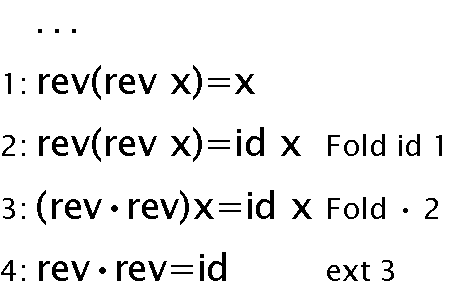
\includegraphics[scale=0.5]{pics/funcprog/revrev=idA}
\caption{Beginning of a proof by substitution of equals}
\label{fig:revrev=idA}
\end{center}
\end{figure}

\begin{figure}
\begin{center}
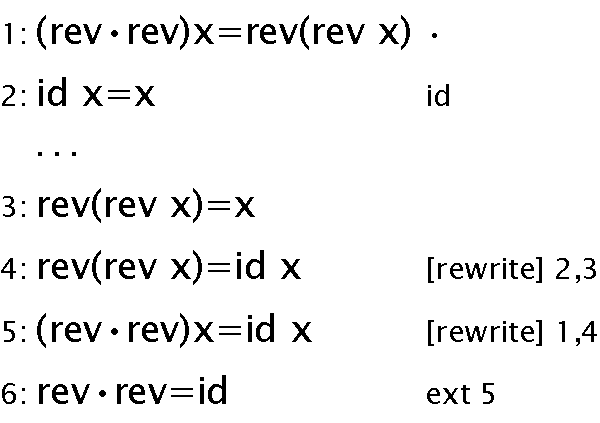
\includegraphics[scale=0.5]{pics/funcprog/revrev=idAunfolded}
\caption{Beginning of a proof by substitution of equals, with hidden steps revealed}
\label{fig:revrev=idAunfolded}
\end{center}
\end{figure}

\Figref{revrev=idA} shows an example proof using this encoding, after two steps. Lines 1, 2 and 3 can be read as a partly-completed equational proof, up the left-hand side and down the right:
\begin{equation*}
\cols[lll]
(\<rev> \bullet \<rev>) x & = \<rev>(\<rev> x) & \reason{$(f \bullet g) \;x = f(g \;x)$}\\
                          & \dots              &\\
                          & = x                &\\
                          & = \<id> x          &\reason{$\<id> x=x$}
\sloc
\end{equation*}

\textsc{Layout} hides antecedents, but they can be revealed: by double-clicking on the justifications of lines 2 and line 3 the hidden steps appear, as shown in \figref{revrev=idAunfolded}.

%\section{Selecting a subformula: \textsc{lethypfind}, \textsc{letconcfind}, \textsc{assoceq} and \textsc{flatten}}
\section{Dealing with associative operators: token selection, Find and Flatten}
\label{sec:funcprog:tokenselection}

\textsc{Letsubstsel} and \textsc{withsubstsel} don't solve all the problems of rewriting, because of associative operators. The problem begins when a formula is input. In Jape's treatment of syntax, just as in any ordinary programming-language compiler, binary operators have relative priorities (or precedences) and an formula such as $A\times B+C$, where \ensuremath{\times} has higher priority than +, is treated internally just like $(A\times B)+C$ but displayed in its unbracketed form.\footnote{Jape tries to keep the user's bracketing structure. If the input is bracketed, so will be the display.} Jape has to be told, faced with the formula $A+B+C$, whether to read it left-associatively as $(A+B)+C$ or right-associatively as $A+(B+C)$ . Whichever you tell it, it will display the result unbracketed as $A+B+C$, and then inevitably some textual segment --- $B+C$ in the left-associative case, $A+B$ in the right-associative --- will look like a subformula but won't be.

You might hope to tell Jape that the operator $+$ is neither left- nor right-associative but \textit{associative} in the mathematical sense, so that $A+B+C$ can be read at will as either $(A+B)+C$ or $A+(B+C)$ as circumstances dictate --- and then you can imagine that it ought to be possible to tell it also that $+$ is commutative, so that $A+B+C$ can be read as $(A+C)+B$ if that is what you wish. That would be pretty difficult, and I never tried very hard to do it. Bernard's encoding tackles the problem head-on, using some specially-coded Jape internals.

\begin{figure}
\centering
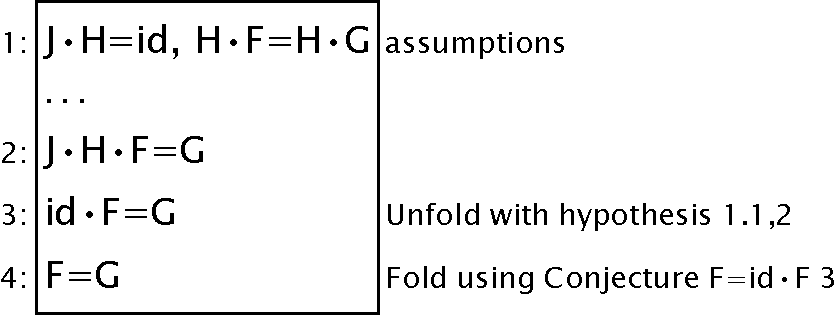
\includegraphics[scale=0.5]{pics/funcprog/assocprobA}
\caption{A problem which involves associativity}
\label{fig:funcprog:assocprobA}
\end{figure}

Consider the function-composition operator ($\bullet$). You can prove --- see the Conjectures panel --- that $(F\bullet G)\bullet H = F\bullet(G\bullet H)$: that is, it's associative. Given the problem in \figref{funcprog:assocprobA}, you might want to extract the $H \bullet F$ subformula of line 2 and rewrite it using the equivalence in the second hypothesis. Unfortunately, $\bullet$ is left-associative (see \texttt{functions\_rules.j}), so that line implicitly reads as $(J\bullet H)\bullet F = G$ and so $H \bullet F$ isn't a subformula. You could, however, transform line 2 into $J\bullet (H \bullet F) = G$ by substitution of equals for equals and the associative equivalence, and then perhaps complete the proof.

The problem is: how can you do this in Jape? Bernard wanted to do it automatically, without the user having to say what equivalence to call upon. (I still wish he hadn't tried, but the price of friendship is that you have to let your friends do what they want to do, and in this case I had to help him do it too.)

\begin{figure}
\centering
\subfigure[subformula selection]{\centering
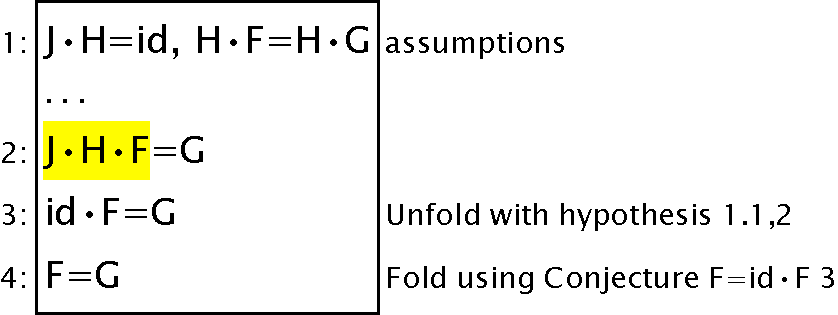
\includegraphics[scale=0.5]{pics/funcprog/subformulaselection}\label{fig:funcprog:subformulaselection}}
\qquad
\subfigure[token selection]{\centering
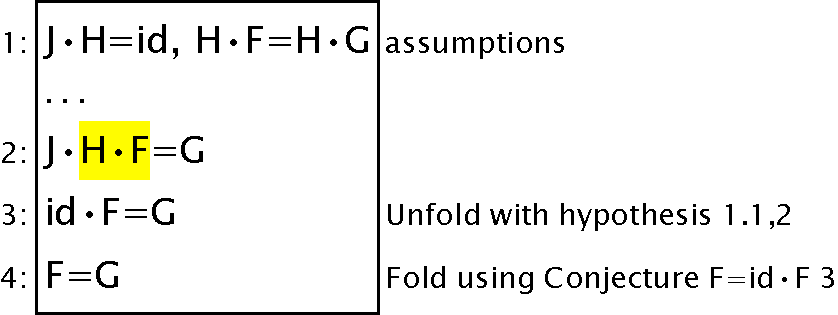
\includegraphics[scale=0.5]{pics/funcprog/tokenselection}\label{fig:funcprog:tokenselection}}
\caption{Alt-press-and-drag across $H \bullet F$}
\label{fig:funcprog:textselectionillustrated}
\end{figure}

\var{id}
Begin with selection. If you try to subformula-select $H \bullet F$ with alt-press-and-drag, Jape doesn't do what you want --- because what you are dragging across isn't a subformula. You first have to switch to a more simplistic form of selection, called token selection, using the Edit menu.\footnote{A token is a single word, like $\<id>$ or $H$, or a connective or a bracket.} Then you can select tokens using alt-press-and-drag, and if you are careful you can select just the sequence of tokens you want, as shown in \figref{funcprog:tokenselection}.\footnote{Token selection is a kind of subformula selection, one in which it's possible to make more mistakes than the normal variety. Jape's internals don't expect subformula selections to deliver proper subformulae, and deliver appropriate error messages when it doesn't.}

\begin{figure}[htbp]
\centering
\subfigure[Find]{\centering
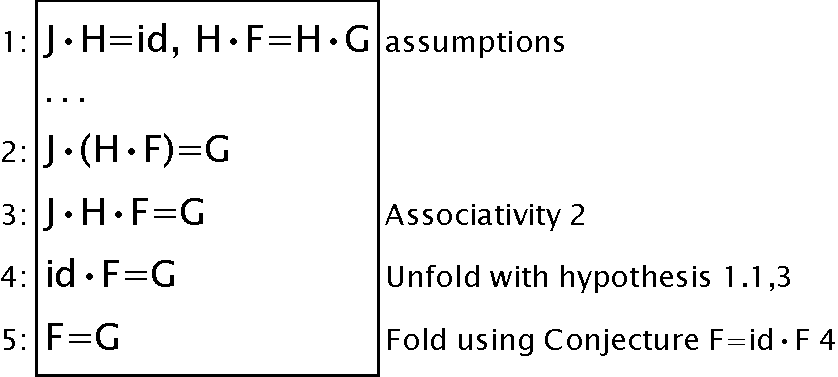
\includegraphics[scale=0.5]{pics/funcprog/assocprobB}\label{fig:funcprog:assocprobB}}
\qquad
\subfigure[unfold]{\centering
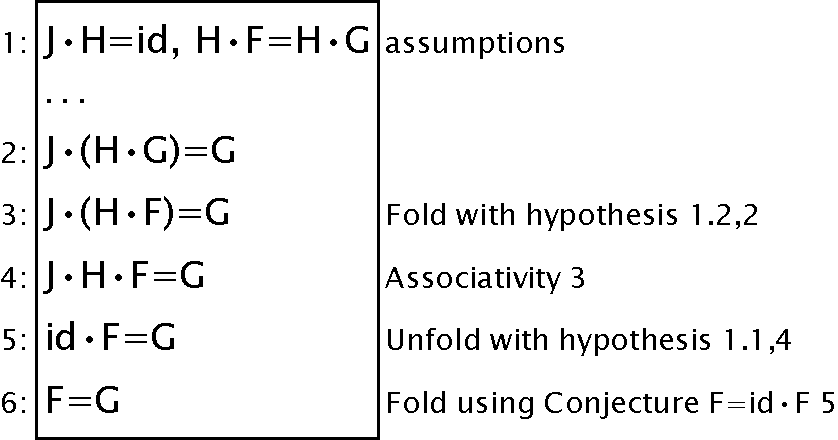
\includegraphics[scale=0.5]{pics/funcprog/assocprobC}\label{fig:funcprog:assocprobC}}
\caption{Token selection and Find allow progress}
\label{fig:funcprog:assocprobBnC}
\end{figure}

With that token-sequence selection you can use Find from the Rules menu or from either of the panels\footnote{I don't think this is good GUI practice, but it's Bernard's encoding.} to rewrite the problem so that $H \bullet F$ is a subformula: the result is \figref{funcprog:assocprobB}, and then Unfold with hypothesis from the Rules menu gives you \figref{funcprog:assocprobC}. Now we're in another hole: we'd like to use the $J\bullet H=\<id>$ equivalence, but $J\bullet H$ isn't a subformula.

\begin{figure}
\centering
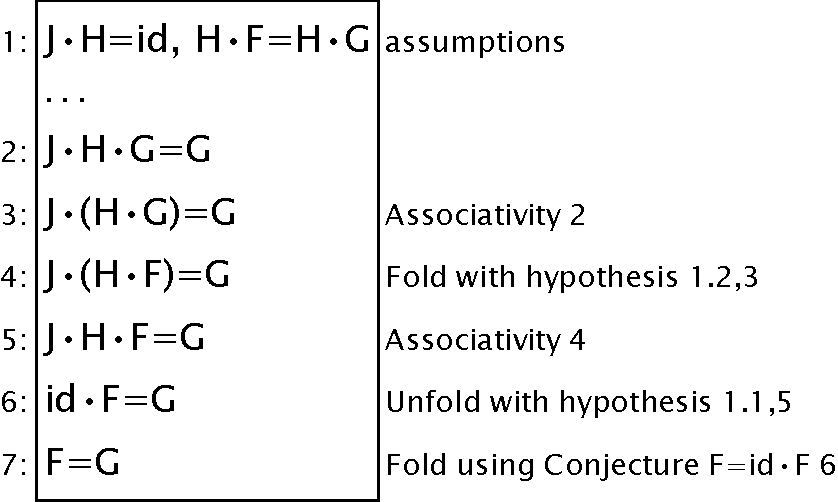
\includegraphics[scale=0.5]{pics/funcprog/assocprobD}
\caption{Flatten takes us out into the open again}
\label{fig:funcprog:assocprobD}
\end{figure}

The solution is to use Flatten (Rules menu or panel) to transform the problem again, taking out brackets from associative formulae where possible. That gives \figref{funcprog:assocprobD}, and the rest is easy. It remains to explain how all this magic works.

The Find entries in menu and panels --- see \texttt{functions\_menus.j} --- simply fire a tactic called FindSelection. That tactic is
\begin{japeish}
TACTIC FindSelection IS \\
\tab WHEN  \\
\tab\tab (LETHYPFIND (\_XOLD=\_YOLD, \_XNEW=\_YNEW) \\
\tab\tab\tab (ALT  \\
\tab\tab\tab\tab (LAYOUT "Associativity" (2) \\
\tab\tab\tab\tab\tab (rewriteHypotheticalEquation \_XOLD \_XNEW \_YOLD \_YNEW) \\
\tab\tab\tab\tab\tab EVALUATE \\
\tab\tab\tab\tab\tab EVALUATE) \\
\tab\tab\tab\tab (LETARGSEL \_XSEL (Fail ("\%s isn't a subterm", \_XSEL))))) \\
\tab\tab (LETCONCFIND (\_XOLD=\_YOLD, \_XNEW=\_YNEW) \\
\tab\tab\tab (ALT \\
\tab\tab\tab\tab (LAYOUT "Associativity" (2) \\
\tab\tab\tab\tab\tab (rewriteEquation \_XOLD \_XNEW \_YOLD \_YNEW) EVALUATE EVALUATE) \\
\tab\tab\tab\tab (LETARGSEL \_XSEL (Fail ("\%s isn't a subterm", \_XSEL))))) \\
\end{japeish}

\textsc{Lethypfind} ($\mathit{oldpat}$, $\mathit{newpat}$) $\mathit{tactic}$ ... and the similar \textsc{letconcfind} tactical are the first part of the magic. They test that: 
\begin{enumerate}
\item the user has made a single subformula or token selection in a hypothesis (\textsc{lethypfind}) or conclusion (\textsc{letconcfind}) formula respectively, dividing it into three sections ($\mathit{before}$, $\mathit{selected}$ and $\mathit{after}$);

\item the original formula unifies with $\mathit{oldpat}$;

\item $\mathit{selected}$ is a valid formula\footnote{Maybe we don't need this condition, but it would be very odd not to impose it.};

\item the text $\mathit{before}$ ( $\mathit{selected}$ ) $\mathit{after}$ is a valid formula;

\item $\mathit{before}$ ( $\mathit{selected}$ ) $\mathit{after}$ unifies with $\mathit{newpat}$.
\end{enumerate}
If all these tests succeed, and if $\mathit{before}$ ( $\mathit{selected}$ ) $\mathit{after}$ is not structurally identical (i.e. identical if you ignore unnecessary brackets) to the original, then the tactic sequence inside the tactical is run. If the tests succeed but the new formula is structurally identical to the old, the tactic sequence isn't run but the tactical still succeeds. That is, \textsc{lethypfind} / \textsc{letconcfind} match, and run their argument tactics, if your text selection reorganises the structure of the formula.

The FindSelection tactic calls either rewriteHypotheticalEquation or rewriteEquation: those rules are%\footnote{The fact that FindSelection splits the selected formula into two, and the rules pick up that split, is an artefact of the way that assoceq is currently implemented; we will fix the problem Real Soon Now. The existence of two rewrite rules, rather than a single one plus a tactic that can use cut, is because Bernard didn't want the kind of trees that result from that kind of simulated forward reasoning --- or perhaps they weren't even invented when he was devising this encoding.}
\begin{japeish}
RULE rewriteEquation(X, X', Y, Y', OBJECT x) IS\\
\tab FROM ASSOCEQ (X, X') AND ASSOCEQ (Y, Y') AND X'=Y' INFER X=Y\\
RULE rewriteHypotheticalEquation(X, X', Y, Y', OBJECT x) IS\\
\tab FROM ASSOCEQ (X, X') AND ASSOCEQ (Y, Y') AND X'=Y'⊦ P INFER X=Y ⊦ P
\end{japeish}

The built-in tactic \textsc{evaluate}, applied to \textsc{assoceq}($E$, $F$), flattens $E$ and $F$ --- that is, removes any internal bracketing, reducing them to a canonical left- or right-associative version as appropriate --- using any relevant theorems / rules / conjectures about associativity, and succeeds if the flattened versions are identical. Each of these rules therefore replaces an equation with a provably equivalent equation. The use of \textsc{layout} in FindSelection hides this internal working and gives Associativity as the justification for the step.

The reverse operation is provided by \textsc{flatten}. The menu and panel entries index the Flatten tactic (see equality\_menus.j)
\begin{japeish}
TACTIC Flatten IS\\
\tab LAYOUT "Associativity" (0)\\
\tab \tab (WHEN\tab (LETARGSEL \_A (FLATTEN \_A))\\
\tab \tab \tab \tab (LETGOAL (\_X = \_Y) (IF(FLATTEN(\_X))) (IF(FLATTEN(\_Y)))) \\
\tab \tab \tab \tab (LETGOAL \_X (FAIL (Cannot Flatten \_X)))\\
\tab \tab )
\end{japeish}

This tactic gives the same justification as FindSelection; via \textsc{flatten} it accesses the same machinery. The argument to flatten is used to determine the principal operator of the formula to be flattened; only subformulae of which that is the operator are flattened.

The effect of all this machinery is to enable the user to manipulate formulae which use associative operators without too many uses of associative rewrite laws.

\var{xs,ys,zs}
\section{Induction}

Jape makes no special treatment of induction. It is handled in the same way as any other logical generalisation rule, using the \textsc{fresh} proviso. Bernard encodes a form of list induction which uses concatenation rather than $\mathit{cons}$:\footnote{Definining lists with concatenation rather than $\mathit{cons}$ has advantages, in particular the fact that it doesn't favour either end of a list when making a reduction. It has difficulties, but it is valid. The sceptics (I am ashamed to admit that I was once one of them!) should note that you can derive this rule from the more familiar $\mathit{cons}$ version. As for evaluation strategies, or function definition by concatenation, that's another story!}
\begin{equation*}
\infer [\reason{(\textsc{fresh} $x$, $\<xs>$, $\<ys>$) listinduction}]
        {\Gamma  |- A(B) }
        {\Gamma  |- A[\,] &
         \Gamma  |- A[x]  &
         \Gamma, A(\<xs>), A(\<ys>) |- A(\<xs>++\<ys>) }
\end{equation*}

That which usually takes two steps (by an induction principle prove $@*\<zs>\cdot A(\<zs>)$, then infer $A(B)$ by specialisation) is collapsed into one. There is no need to introduce quantification into equational reasoning, and the one-step rule is perfectly convenient. Bernard encodes it directly:
\begin{japeish}
RULE listinduction (B, OBJECT x, OBJECT xs, OBJECT ys, ABSTRACTION A) \\
\tab WHERE FRESH x, xs, ys IS\\
\tab \tab FROM A[] AND A[x] AND A xs, A ys ⊦ A(xs++ys) INFER A(B)
\end{japeish}

Sometimes you will want to make a proof by induction of a proposition which is expressed in terms of some variable or other, and then you would want induction to apply to every instance of that variable. Other times you may want to be more precise in specifying just what instances of what sub-formula are to be the basis of induction, and so we require the user to specify those instances. Bernard could have allowed both mechanisms, activated by different entries in a menu, but has instead required you always to select the particular instances of a subformula which you wish to be the subject of induction. The entry in the menu which gives the user access to the list induction principle connects to a tactic which uses the letsubstsel/withsubstsel mechanism:
\begin{japeish}
TACTIC "list induction tactic" IS \\
\tab WHEN \\
\tab\tab (LETSUBSTSEL \_A (WITHSUBSTSEL listinduction))\\
\tab\tab (FAIL(Please select a sub-formula on which to perform induction))
\end{japeish}

\var{map}
\section{Controlling collections of rules}

In functional programs each function definition corresponds to a number of individual statements of equality. The definition of $\<map>$, for example, gives three:
\begin{equation*}
\cols[lllll]
	\<map> & f & [\,] & = & [\,] \\
	\<map> & f & [x] & = & f\,x \\
	\<map> & f & (\<xs>++\<ys>) & = & \<map>\,f\,\<xs> ++ \<map>\,f\,\<ys>
\sloc
\end{equation*}


It would be tedious to be required to give a name to each individual equality, and in any case Bernard expects his users to be happy to refer to them as a collection --- ``use one of the $\<map>$ equalities'', rather than ``use the $\<map>$ equality which applies to singletons''.

The \textsc{rules} directive allows us to make and name collections of rules. If we turn all the function definitions into collections we can use them, with some instantiation of their variables, to close the left-hand antecedent of a \textit{rewrite} rule application or to close a tip of a proof tree in the normal way. The definition of \texttt{map}, for example, goes as follows:
\begin{japeish}
RULES map\\
\tab ARE map F [] = []\\
\tab AND map F [X]= [F X]\\
\tab AND map F (Xs++Ys) = map F Xs ++ map F Ys\\
END
\end{japeish}
This generates three rules, called \texttt{map'0}, \texttt{map'1} and \texttt{map'2}, plus a tactic \texttt{map}:
\begin{japeish}
TACTIC map IS ALT map'0 map'1 map'2
\end{japeish}

In addition, for control of searching of the collections of rules, Bernard groups them into collections called `theories'. Part of the \texttt{List} theory, for example, as it is given in \texttt{functions\_rules.j} is
\begin{japeish}
THEORY List IS\\
\tab RULES length \\
\tab ...\\
\tab RULE\tab none  IS none X\tab = [ ]\\
\tab RULE\tab one IS one X\tab = [X]\\
\tab RULE\tab cat IS cat = fold (++) []\\
\tab RULES rev\\
\tab ...\\
\tab RULES ++\\
\tab ...\\
\tab RULES map\\
\tab ...\\
\tab RULE filter IS filter P = cat • map (if P (one, none))\\
\tab RULES zip\\
\tab ...\\
\tab RULES fold \\
\tab ...\\
\tab RULE rev2 IS rev2 = fold rcat [] • map one\\
\tab RULE rcat IS rcat Xs Ys = Ys ++ Xs\\
\tab RULE ":" IS X:Xs = [X] ++ Xs\\
END
\end{japeish}

The effect of \textsc{theory} is to define all the rules and tactics described by its components, plus a tactic which allows search of those components. In this case the tactic is
\begin{japeish}
TACTIC List IS ALT length none rev (++) map filter zip fold rev2 rcat (:)
\end{japeish}

\begin{figure}
\begin{center}
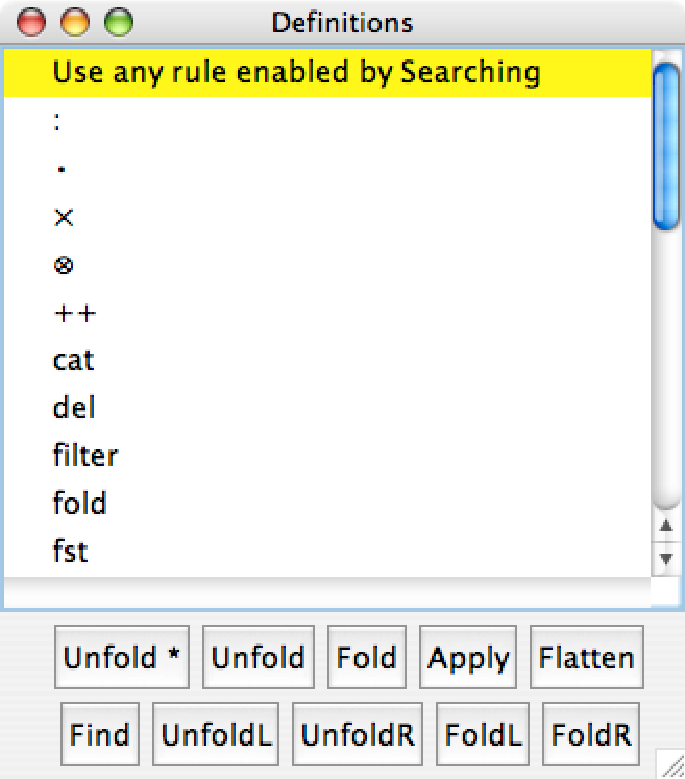
\includegraphics[scale=0.5]{pics/funcprog/definitionspanel}
\caption{The functional programming panel of definitions}
\label{fig:funcprog:definitionspanel}
\end{center}
\end{figure}

The rule-collections --- but not the theory-collections --- are put into a panel of definitions. The panel is described in \texttt{functions\_menus.j} as
\begin{japeish}
TACTICPANEL "Definitions" \\
\tab TACTIC "Use any rule enabled by Searching" IS SearchTactic\\
\tab ENTRY ":"\\
\tab ENTRY "•" \\
\tab ENTRY "×" \\
\tab ENTRY "⊗" \\
\tab ...\\
\tab BUTTON "Unfold *" IS apply RepeatedlyUnfold\\
\tab PREFIXBUTTON "Unfold" IS apply UnfoldObvious\\
\tab PREFIXBUTTON "Fold" IS apply FoldObvious\\
\tab PREFIXBUTTON "Apply" IS apply\\
\tab BUTTON "Flatten" IS apply Flatten\\
\tab BUTTON "Find" IS apply FindSelection\\
END
\end{japeish}
This produces the panel shown in \figref{funcprog:definitionspanel}. I discuss the effect of the tactics bound to the buttons and entries in what follows.

\section{Searching collections of rules and theorems}

It's quite possible, using the Unfold and Fold buttons on the Definitions panel, plus the Unfold with hypothesis and Fold with hypothesis entries in the Rules menu, to construct proofs entirely by hand --- selecting the subformula to be replaced, the definition or hypothesis to be used, pressing the appropriate button or choosing the appropriate menu entry. But it's also quite easy to program Jape to do a sort of evaluation step. This involves identifying helpful equations (in the form of rules or theorems) which can be used to rewrite part of the conclusion of the problem sequent.

Jape has a number of built-in mechanisms which help with the process. The \textsc{alt} tactical allows an undirected search amongst a number of possibly-applicable tactics, and I have illustrated above how the rules and theory directives automatically construct \textsc{alt}s which may be useful in searching for a proof. But in equational reasoning the problem is somewhat different: we are looking for a subformula which is replaceable and a definition or hypothesis which matches it; \textsc{alt} is not sufficient to do the job.

Jape's support for search in equational reasoning is at present the \textsc{fold}, \textsc{unfold}, \textsc{foldhyp} and \textsc{unfoldhyp} tacticals. \textsc{Fold} and \textsc{unfold} tacticals take a rewrite rule and an \textsc{alt} tactic, which is treated as a collection of rules. They filter the rules to consider only those whose consequents have a conclusion of the form $L\;\mathit{op}\;R$ for some formulae $L$ and $R$ and a binary operator $\mathit{op}$;\footnote{The rules --- actually rules and theorems --- are doubly filtered because Jape eliminates all unproved conjectures unless the \texttt{applyconjectures} variable is set \texttt{true}.} they search for subformulae of the conclusion of the problem sequent which match the $R$ (\textsc{fold}) or $L$ (\textsc{unfold}) of one of the rules, and when they find a coincidence try to apply the rewrite rule followed by the matching filtered rule. \textsc{Foldhyp} and \textsc{unfoldhyp} are similar, except that they take a pattern which allows the user to define $\mathit{op}$, and they search the list of current hypotheses rather than a collection of rules.

Although distressingly ad-hoc in my opinion (I'd rather Jape was more purely a logic engine), these techniques are fast and they work well. In this encoding the rules are such that automatic \textsc{fold}ing is little use: too many equalities have right-hand sides which are similar, and searching with alt for a match rarely finds a useful one. But automatic \textsc{unfold}ing can often be fruitful: if there is a subformula which matches $\<map>\; F\; (\mathit{Xs}++\mathit{Ys})$, for example, then unfolding with the rule $\<map>\; F\; (\mathit{Xs}++\mathit{Ys}) = \<map>\; F\; \mathit{Xs}++ \<map>\; F\; \mathit{Ys}$ is probably worthwhile.

Bernard's search mechanism, then, is based on the tactic
\begin{japeish}
TACTIC Unfold(x) IS LAYOUT "Fold \%h" (1) (UNFOLD rewrite x)
\end{japeish}

which is given an alt tactic \texttt{x} and which searches for (backwards) \textsc{unfold} actions which it can carry out by rewriting with the rules within \texttt{x}.

The magic by no means stops with the unfold tactical, because Bernard also uses the collections of theories to control the search. The idea is that you should be able to `turn on and off' the definitions and theorems in particular theories when searching. Because the variable-processing facilities of Japeish are primitive, this has to be done using radiobuttons in a special Searching menu.

Bernard grouped the equality rules into three theories: List (illustrated above), Functions and Reflect. He also grouped conjectures into collections, some of which Jape can be made to search. Here, for example, is the Listthms collection:
\begin{japeish}
THEOREMS ListThms\\
ARE\tab rev • rev\tab = id\\
AND\tab rev2\tab = rev\\
AND\tab map F • map G\tab = map (F • G)\\
AND\tab map F • cat\tab = cat • (map (map F))\\
AND\tab none • F\tab = none\\
AND\tab map F • none\tab = none\\
AND\tab map F • one\tab = one • F\\
AND\tab map F • rev\tab = rev • map F\\
AND\tab map id\tab = id\\
AND\tab length•map F\tab = length\\
AND\tab zip • (map F ⊗ map G)\tab = map (F⊗G)\\
AND\tab map F • if P (G,G')\tab = if P (map F • G, map F • G')\\
AND\tab filter P\tab = map fst • filter snd • zip • (id ⊗ map P)\\
END
\end{japeish}

These, once proved, can be searched when automatically unfolding equalities; they can even be searched before they are proved, if applyconjectures is set to true.

The basic technique at present is a hack to get around the fact that Jape doesn't yet have any analogue of the ML \textit{case} expression, which could be used to direct the activity of a tactic according to the value of a variable.\footnote{It probably took longer to type this footnote than to implement the mechanism --- but the manual must come first!} The hack is to use variables each of which is set to the name of a theory if we want to search that theory, or to the name of a tactic which is certain to fail, if we don't want to search it. The justfail tactic is
\begin{japeish}
TACTIC JUSTFAIL IS (ALT)
\end{japeish}
and the Searching menu is
\begin{japeish}
MENU "Searching" IS\\
\tab RADIOBUTTON dohyp IS \\
\tab "Search hypotheses" IS DoHyp\\
\tab AND "Ignore hypotheses" IS JUSTFAIL\\
\tab INITIALLY DoHyp\\
\tab END \\
\\
\tab RADIOBUTTON list IS \\
\tab "List rules enabled" IS List\\
\tab AND\tab "List rules disabled" IS JUSTFAIL\\
\tab INITIALLY List\\
\tab END
END \\
...
\end{japeish}

The Auto tactic is set up either to unfold or to fold --- though for the reasons given above, it's never much used for folding --- and is defined as
\begin{japeish}
TACTIC Auto(foldunfold, foldunfoldhyp) IS \\
ALT\tab (dohyp foldunfoldhyp)\\
\tab (foldunfold list) \\
\tab (foldunfold listthms) \\
\tab (foldunfold function) \\
\tab (foldunfold functionthms) \\
\tab (foldunfold reflect) \\
\tab (foldunfold reflectthms)\\
\tab (FAIL (Cannot find anything to foldunfold))
\end{japeish}
It's called from the Unfold * button with the tactic
\begin{japeish}
SEQ\tab (Auto Unfold UnfoldWithAnyHyp) \\
\tab (DO (Auto Unfold UnfoldWithAnyHyp))
\end{japeish}
--- since \textsc{do} always silently succeeds, Bernard wanted to make the button fail noisily if there was nothing at all that it could do; hence the double invocation of the tactic.

He uses the same tactic --- but only singly, without repetition --- if you double-click on a conclusion:
\begin{japeish}
CONCHIT C IS Auto Unfold UnfoldWIthAnyHyp
\end{japeish}

The remaining parts of the jigsaw are the UnfoldWithAnyHyp tactic
\begin{japeish}
TACTIC UnfoldWithAnyHyp IS UNFOLDHYP "Fold with hypothesis" (\_A=\_B)
\end{japeish}
and the Fold/Unfold with hypothesis pair of rules:
\begin{japeish}
RULE "Fold with hypothesis" (X, OBJECT x) IS \\
\tab\tab FROM X=Y ⊦ AA[x{\textbackslash}Y] INFER X=Y ⊦ AA[x{\textbackslash}X]\\
RULE "Unfold with hypothesis" (Y,OBJECT x) IS \\
\tab\tab FROM X=Y ⊦ AA[x{\textbackslash}X] INFER X=Y ⊦ AA[x{\textbackslash}Y]
\end{japeish}
These rules are named for forward reading, so the menu entries which enable them to be used by hand have to be labelled contrariwise.

All of the other techniques that we have used have been discussed in earlier chapters, with the exception of the next, which is novel.

\section{Transitive reasoning: \texttt{trfunctions.jt}} 

There's a structural analogy between the logical cut rule and the rule of transitive equality:
\begin{ruletab}{|l|l|}
\hline
$\infer[\reason{cut}]
       {\Gamma|-C}
       {\Gamma|-B & \Gamma,B|-C}$
&
$\infer[\reason{$=$ transitive}]
       {\Gamma|-A=C}
       {\Gamma|-A=B & \Gamma|-B=C}$\\
\hline
\end{ruletab}
Each produces a formula $B$ on the right-hand side in one antecedent, and deploys it on the left in the other. In a cut the movement is from one side of the turnstile to the other; in transitivity it's from one side of an equality to the other.

There's an analogy, too, between logical axiom (hyp in \chapref{ItL} and this chapter) and reflexive equality:
\begin{ruletab}{|l|l|}
\hline
$\infer[\reason{hyp}]
       {\Gamma,C|-C}
       {}$
&
$\infer[\reason{$=$ reflexive}]
       {\Gamma|-C=C}
       {}$\\
\hline
\end{ruletab}

\begin{figure}
\begin{center}
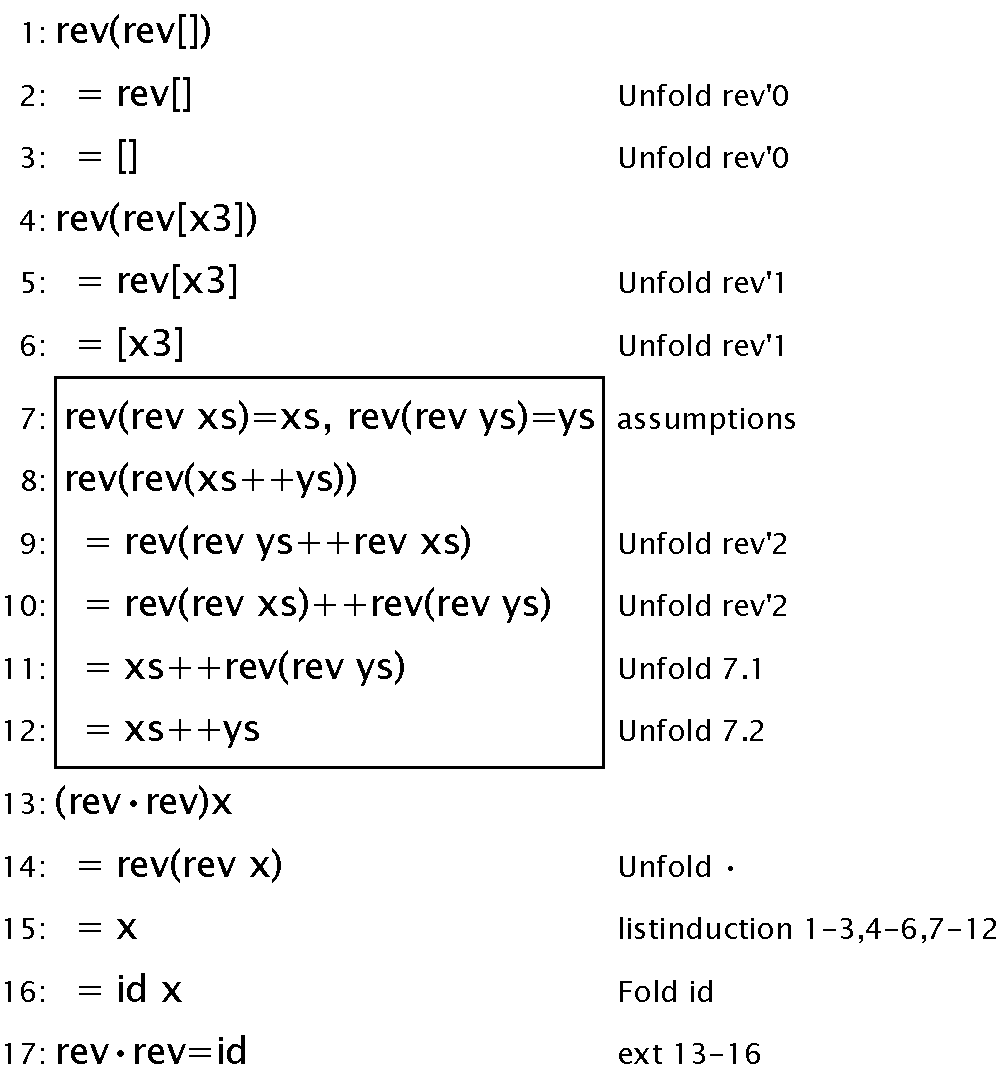
\includegraphics[scale=0.5]{pics/funcprog/revrev=idtransitively}
\caption{A proof of $\protect\<rev>\bullet\protect\<rev>=\protect\<id>$ exploiting transitivity and reflexitivity}
\label{fig:funcprog:revrev=idtransitively}
\end{center}
\end{figure}

\begin{figure}
\begin{center}
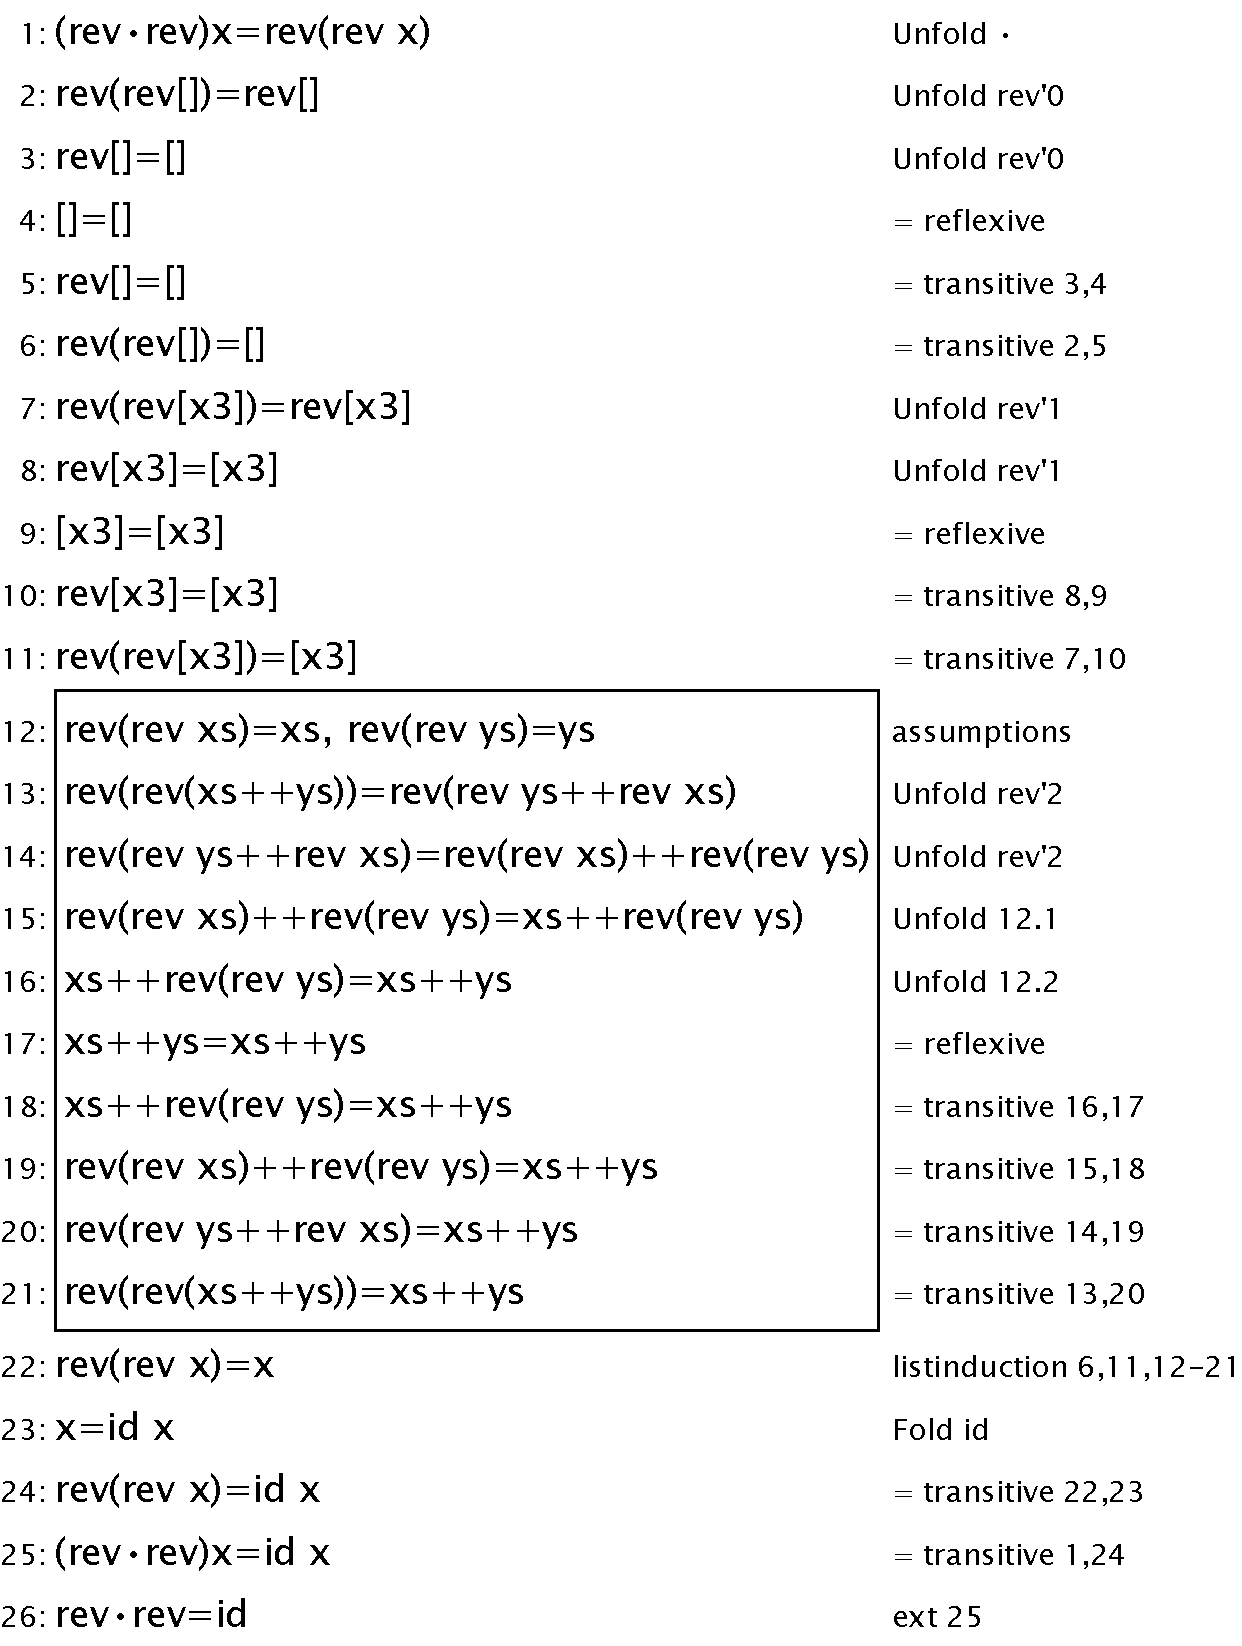
\includegraphics[scale=0.5]{pics/funcprog/revrev=idtransitivelyrevealed}
\caption{A proof of $\protect\<rev>\bullet\protect\<rev>=\protect\<id>$ with transitive and reflexive steps revealed}
\label{fig:funcprog:revrev=idtransitivelyrevealed}
\end{center}
\end{figure}

\Chapref{ItL} shows that you can make a box-and-line version of a tree by recognising instances of hyp, and make it more powerful by recognising instances of cut. The same can be done with transitivity and reflexivity, producing proofs much more like the ones that equality-reasoners like to deal with. For example, \figref{funcprog:revrev= idtransitively} shows a proof that $\<rev>\bullet\<rev>=\<id>$. Apart from details of layout, the steps on lines 1-3, 4-6, 8-12 and 13-16 look just like the equational proofs in Bird and Wadler. Much of the trickery is hiding of transitive and reflexive equality steps, and the same proof with that part of its machinery exposed is shown in \figref{funcprog:revrev=idtransitivelyrevealed}.

Proofs like that are made by working on one side or the other of an equality. Jape needs to know that it's equality we care about. \texttt{functions.jt} already contains declarations of the rules:
\begin{japeish}
AUTOMATCH "= reflexive" \\
TRANSITIVE  "= transitive" \\
REFLEXIVE "= reflexive" \\
\end{japeish}
and \texttt{functions\_menus.j} puts a checkbox in the Edit menu:
\begin{japeish}
CHECKBOX hidetransitivity "transformational style" INITIALLY false
\end{japeish}
Now \texttt{functions\_transitivity.j}, invoked from \texttt{trfunctions.jt}, rubs it in and makes both the display-controlling variables true:
\begin{japeish}
INITIALISE hidereflexivity true \\
\\
MENU Transitivity IS \\
\tab CHECKBOX  hidetransitivity \\
\tab\tab "Transitive Presentation Style" \\ 
    INITIALLY true \\
END \\
\end{japeish}
In the same file Bernard adds entries to menus and buttons to panels to allow reductions on one side or the other of an equality\footnote{Bernard prefers to work with the variable \texttt{autoselect} set true, and strum on buttons in panels --- he invented panels just so he could do that! I prefer to work by pointing at the thing I'm going to work on, so in my encodings I set \texttt{autoselect} false, and in transitivity settings I use the \textsc{letlhs} / \textsc{letrhs} tacticals to let Jape find out what I'm up to. Horses for courses.}
\begin{japeish}
TACTICPANEL Definitions  \\
\tab BUTTON  "Flatten LHS"   IS apply FlattenLHS \\
\tab BUTTON  "Flatten RHS"   IS apply FlattenRHS \\
\tab BUTTON  "Unfold LHS"    IS apply UnfoldL COMMAND \\
\tab BUTTON  "Unfold RHS"    IS apply UnfoldR COMMAND \\
\tab BUTTON  "Fold LHS"  IS apply FoldL   COMMAND \\
\tab BUTTON  "Fold RHS"  IS apply FoldR   COMMAND  \\
END \\
\\
MENU Unfolding IS \\
\tab ENTRY "Unfold LHS"     IS (UnfoldL SearchTactic) \\
\tab ENTRY "Unfold RHS"     IS (UnfoldR SearchTactic) \\
\tab ENTRY "Fold LHS"       IS (FoldL SearchTactic) \\
\tab ENTRY "Fold RHS"       IS (FoldR SearchTactic) \\
\tab ENTRY "Flatten LHS"    IS FlattenLHS \\
\tab ENTRY "Flatten RHS"    IS FlattenRHS \\
END
\end{japeish}
Most of the gesture-interpreting work is down to UnfoldR and UnfoldL. This is how UnfoldL begins:
\begin{japeish}
TACTIC UnfoldL(rule) IS \\
\tab (WHEN  \\
\tab \tab (LETSUBSTSEL (\_A\{\_x{\textbackslash}\_F\}=\_B)       /* Rewrite the selection */ \\
\tab \tab \tab "= transitive"  \\
\tab \tab \tab (LAYOUT "Unfold \%h" ()  \\
\tab \tab \tab \tab (rewriteLR\{X,AA,x{\textbackslash}\_F,\_A,\_x\})  \\
\tab \tab \tab \tab (USEHYPORRULE rule)))
\end{japeish}
--- if you've made a selection on the left of the equality, run rewriteLR on it, and label the result with the name of the rule. (The use of argument-substitution in the call of rewriteLR may be an attempt to deal with the consequences if the selection is on the right of the equality, but I think \textsc{withsubstsel} would be a better mechanism to use. But then, I've tinkered enough with this encoding: leave it as it is.) The rewrite tactic it uses is one of a pair from \texttt{equality\_rules.j}
\begin{japeish}
RULE rewriteLR (OBJECT x) IS FROM X=Y INFER AA\{x{\textbackslash}X\}=AA\{x{\textbackslash}Y\} \\
RULE rewriteRL (OBJECT x) IS FROM X=Y INFER AA\{x{\textbackslash}Y\}=AA\{x{\textbackslash}X\} /* derivable */
\end{japeish}
and \texttt{functions\_transitivity.j} has
\begin{japeish}
TACTIC USEHYPORRULE(rule) IS (WHEN (LETHYP \_H (WITHHYPSEL hyp)) (ALT hyp rule))
\end{japeish}

The second UnfoldL alternative is 
\begin{japeish}
(LETCONCFIND (\_XOLD=\_YOLD, \_XNEW=\_YNEW) \\
\tab (LETGOALPATH G \\
\tab \tab "= transitive"  \\
\tab \tab (ALT  \\
\tab \tab \tab (LAYOUT "Associativity" (2) \\
\tab \tab \tab \tab (associativity \_XNEW \_XOLD) EVALUATE) \\
\tab \tab \tab (LETARGSEL \_XSEL (Fail ("\%s isn't a subterm", \_XSEL))))))
\end{japeish}
--- if you've made a token selection which isn't a subformula, do the \textsc{assoceq} thing.

The third UnfoldL alternative is 
\begin{japeish}
(LETHYP (\_A=\_B)  /* Use selected hypothesis to rewrite everywhere */ \\
\tab (LETCONC (\_X=\_Y) \\
\tab \tab "= transitive"  \\
\tab \tab (ALT \\
\tab \tab \tab (LAYOUT "Unfold" ALL (rewriteLR\{X{\textbackslash}\_A\}) (WITHHYPSEL hyp)) \\
\tab \tab \tab (Fail "Cannot use the selected hypothesis to unfold on the LHS"))))
\end{japeish}
--- if you've selected a hypothesis, use it left-to-right to rewrite the conclusion.

The penultimate UnfoldL alternative is the tricky one. It searches the left-hand side for things to work on:
\begin{japeish}
(LETGOAL (\_A=\_B)                      /* No selection: a little automation */ \\
\tab (LETGOALPATH G \\
\tab \tab "= transitive" \\
\tab (ALT (UNFOLDWITH1 rule)             /* Close with the rule */ \\
\tab \tab (UNFOLDWITH2 FunSearch4 rule)  /* Close by rewriting inside the formula */ \\
\tab \tab (Fail "Nothing obvious to unfold on the LHS")) \\
\tab (GOALPATH (SUBGOAL G 1)))) \\
\end{japeish}
UNFOLDWITH1 is straightforward:
\begin{japeish}
TACTIC UNFOLDWITH1(rule1) IS (LAYOUT "Unfold \%s" () rule1) 
\end{japeish}
\%s in the string is replaced by the label of the root of the tree produced by rule1.

UNFOLDWITH2 is more complicated, because of what Funsearch does. Here's the bundle of rules it uses:
\begin{japeish}
RULE FunctionOperand  IS FROM X=Y  INFER F X = F Y \\
RULE FunctionOperator IS FROM F=G  INFER F X = G X \\
RULE LeftPair         IS FROM X=X' INFER (X, Y)=(X', Y) \\
RULE RightPair        IS FROM Y=Y' INFER (X, Y)=(X, Y') \\
RULE Singleton        IS FROM Y=Y' INFER [Y]=[Y']
\end{japeish}
and here's the bundle of search tactics:
\begin{japeish}
TACTIC FunApply(rule) IS (rule) \\
\\
TACTIC FunRecurse(continue, rule) IS \\
\tab (ALT (continue rule) \\
\tab \tab (LAYOUT "\%h" ()  FunctionOperator (continue rule)) \\
\tab \tab (LAYOUT "\%h" ()  FunctionOperand  (continue rule)) \\
\tab \tab (LAYOUT "\%h" ()  LeftPair         (continue rule)) \\
\tab \tab (LAYOUT "\%h" ()  RightPair        (continue rule)) \\
\tab \tab (LAYOUT "\%h" ()  Singleton        (continue rule))) \\
\\
TACTIC FunSearch1(rule) IS (FunRecurse FunApply rule) \\
TACTIC FunSearch2(rule) IS (FunRecurse FunSearch1 rule) \\
TACTIC FunSearch3(rule) IS (FunRecurse FunSearch2 rule) \\
TACTIC FunSearch4(rule) IS (FunRecurse FunSearch3 rule) \\
\end{japeish}
Each of the steps hides its own action with \%h, effectively transmitting its child action label down the tree. Finally, UNFOLDWITH2 has to do a little \textsc{goalpath} dance, switching from the final position (G1) to the original position (G), labelling it --- \textsc{layout} is like an assignment to a tree node -- and then switching back to G1, to make sure that the correct layout is applied to the root of the tree that it builds:
\begin{japeish}
TACTIC UNFOLDWITH2(rule1, arg) IS \\
\tab /* override any layout set by rule1 */ \\
\tab (LETGOALPATH G \\ 
\tab \tab (rule1 arg) \\ 
\tab \tab (LETGOALPATH G1
\tab \tab \tab (GOALPATH G) \\ 
\tab \tab \tab (LAYOUT "Unfold \%h" ()) \\ 
\tab \tab \tab (GOALPATH G1)))
\end{japeish}
 
Finally, if nothing works, the last alternative in UnfoldL gives an error message:
\begin{japeish}
(Fail (Cannot unfold LHS because there is no equation)))
\end{japeish}

And that's how it works: quite remarkably simple in the end.